\chapter{Background}
%Before explaining the proposed VA design, the background information necessary to understanding VA architecture is described %briefly, followed by a short summary of state-of-art algorithms for object detection used in our proposed VA.
Object detection in images and videos has received a lot of attention in the computer vision and video analytics communities in recent years. There are many different approaches to video moving object detection, both utilizing compressed and uncompressed data. In this chapter, we briefly introduce the state-of-the-art approaches for moving object detection on both compressed domain and pixel domain. In addition, the background information necessary to understanding VA architecture is described briefly.
\section{Surveillance Video Analytics Architectures and Challenges}
\begin{figure*}
\centering
\subfloat[]
{
    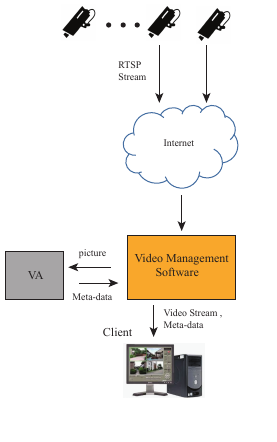
\includegraphics[scale=0.6]{Figures/Va-neta.png}
    \label{fig:va_a}
}
\subfloat[]
{
    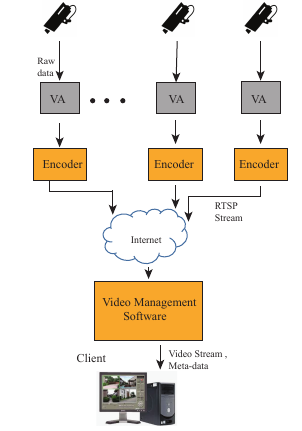
\includegraphics[scale=0.6]{Figures/Va-netb.png}
    \label{fig:va_b}
}
\caption{Video Analytics Implementation, (a) Video management server based implementation, (b) Edge camera based implementation}
\label{fig:va_arch}
\end{figure*}
Video surveillance systems are typically built using the following main components: surveillance cameras, VMS, storage and VA modules (optional). VA can be implemented in two main configurations, as discussed below.
\subsection{Edge Camera Based Implementation}
In this approach, the VA is implemented through a  camera device or video encoder \cite{chen2017smart} such as that shown in Figure \ref{fig:va_b}, which must have sufficient processing power to run the VA functionality. Hence it is an expensive and challenging approach to wide-area video processing. On the surface, this approach seems otherwise ideal, however it does not perform satisfactorily in many cases as it imposes limitations on the overall surveillance system design and performance. Most camera device still lack sufficient processing power for highend VA requirements, and therefore, this approach has many drawbacks in real-world deployment. 
\subsection{Video Management Server Based Implementation}
In this approach, as shown in Figure \ref{fig:va_a}, VA is implemented through a dedicated server that pulls the video from the camera devices or from VMS, analyzes it, and issues analysis results. However, it has some challenges, which are listed below:
\begin{itemize}
\item The VA server requires the video to be transmitted and therefore causes an increase in network traffic. In detail, running video analytics by streaming all video to the cloud conflicts with the bandwidth constraints of some deployments, which preclude uploading all camera data. Each camera’s uplink bandwidth is limited, both by the physical constraints of modern wide-area network infrastructure and the monetary cost of operating a widespread camera deploy-
ment. Specifically, we consider large-scale deployments where each camera receives a bandwidth allocation of a few hundred kilobits per second, or less. For comparison, a low-quality H.264-encoded 1080p (1920×1080 pixels) stream is approximately two Mb/s, an order of magnitude greater than our available uplink bandwidth. Yet, such low-quality data is often insufficient to perform accurate analysis: Modern 4K (3840×2160 pixels) cameras produce up to 30-40 Mb/s, two
orders of magnitude beyond the uplink bandwidth, and this
gap will only expand as 8K (7680 × 4320 pixels) cameras become more common. As a concrete example, we have an off-campus deployments where cameras are mounted next
to traffic lights at an intersection. The local internet service provider charges \$400 per month for a single 35 Mb/s uplink, creating a strong economic incentive for us to share that bandwidth between as many cameras as possible (currently,
eight 4K cameras share each uplink).This bandwidth gap, exacerbated by the requirement for high-quality data, necessitates an edge-based decision about
which frames to send to the datacenter. An edge-based filter answers this challenge with semantic filtering that uploads only frames that are relevant to applications.
\item The video quality being analyzed by the VA server is usually degraded because of compression and transmission effects, and therefore, the VA performance may be compromised.
\item The VA server is limited by its processing power, which makes it infeasible for large scale surveillance installations which deploy hundreds (and increasingly thousands) of cameras requiring a variety of VA functionalities. For example, a 1920 × 1080 pixel stream at 30 frames per second is $\approx$ 1.5 Gb/s when decompressed. Accomplishing VA at scale requires abundant compute, memory, and storage resources, so existing systems often perform this processing in the cloud, using GPUs.
\end{itemize}
However, this approach is independent of video cameras, and is therefore applicable to most types of surveillance systems, and recent technological developments can reduce the effect of the above drawbacks. For example, the release of high definition video surveillance footage with resolutions up to 1080p will decrease the impact of the image quality degradation during codec processing and by releasing the new video coding standard as well as the transcoder \cite{thanh2019efficient}, high efficiency video coding (HEVC)\cite{sullivan2012overview} which has achieved approximately twice the standard compression\cite{ohm2012comparison} will decrease traffic in the network and at the central server, where powerful devices will have sufficient processing power to handle hundreds of camera. Moreover, some edge-based filtering approaches that
is designed to overcome these above issues \cite{canel2019scaling}\cite{li2020reducto}\cite{chen2015glimpse}. These approaches use edge-compute resources collocates with the cameras to identify the video sequences that are most relevant to datacenter applications (“filtering”) and offloads only that data for further analysis (“forwarding”). In this way, it supports near-real-time processing running in datacenters while limiting the use of low-bandwidth wide-area network links. In this study, we present an edge-based filter, a system that offers the benefits of both edge computing and datacenter-centric approaches to wide-area video processing.
\subsection{Video Codec and Video Coding Motion Vectors}
\subsubsection{Video Codec}
\begin{figure*}
\centering
 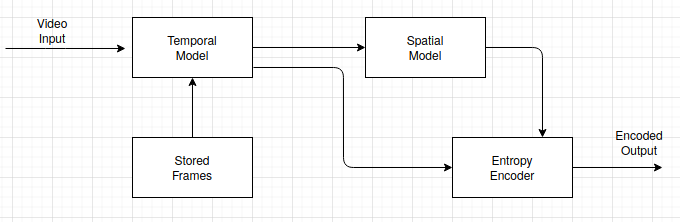
\includegraphics[width=0.8\linewidth]{Figures/encoder.png}
 \caption{Video encoder block diagram.}
 \label{fig:encoder}
\end{figure*}
The traditional video coding standards, such as MPEG-1, MPEG-2, H.264 and H.265, are based on block-based motion compensation, transform, quantisation and entropy coding. A video encoder as shown in Figure \ref{fig:encoder} consists of three main functional units: a temporal model, a spatial model and an entropy encoder. The input to the temporal model in an uncompressed video sequence. The temporal model attempts to reduce temporal redundancy by exploiting the similarities between neighbouring video frames, usually by constructing a prediction of the current video frame. In MPEG-4 Visual and H.264, the prediction is formed from one or more previous of future frames and is improved by compensating for differences between the frames (motion compressed prediction). The output of the temporal model is a residual frames (created by subtracting the prediction from the actual current frame) and a set of model parameters, typicially a set of MVs describing how the motion was compressed. \\
The residual frame formes the input to the spatial model which makes use of similarities between neighbouring samples in the residual frame to reduce spatial redundancy. In MPEG-4 Visual and H.264 this is archieved by applying a transform to the residual samples and quantizing the results. The transform converts the samples into another domain in which they are represented by transform coefficients. The coefficiencents are quantised to remove insignificant values, leaving a small number of significant coefficients that provide a more compact representation of the residual frame. The output of the spatial model is a set of quantised transform coefficients.\\
The parameters of the temporal model (typically MVs) and the spatial model (coefficients) are compressed by the entropy encoder. The removes statistical redundancy in the data (for example, representing commonly-occurring  vectors and coefficients by short binary codes) and produces a compressed bitstream or file that may be transmitted and/or stored. A compressed sequency consists of coded motion vector parameters, coded residual coefficients and hear information.\\
The video decoder reconstructs a video frame from the compressed bitstream. The coefficients and motion vectors are decoded by an entropy decoder after which the spatial model is decoded to reconstruct a version of the residual frame. The decoder uses the motion vector parameters, together with one or more previously decoded frames, to create a prediction of the current frame and the frame itself is reconstructed by adding the residual frame to this prediction.
\subsubsection{Video Coding Motion Vectors and Blocked-based Motion Estimation}
	Changes between video frames may caused by object motion (regrid object motion, for example a moving car, and deformable object motion, for example a moving arm), camera motion (panning, tilt, zoom, rotation) and lighting changes. With the exception of uncovered regions and lighting changes, these differences coresspond to pixel movements between frames. It is possible to estimate the trajectory of each pixel between successive video frames, producing a field of pixel trajectories known as optical flows. In simple terms, optical flow gives the measure of movement of a pixel or a block in two consecutive frame. This measure of movement is given in the form of a vector where the magnitude of the vector signifies the amount of motion and the angle of the vector specifies the direction of the motion. This vector is called motion vector. 
\begin{figure*}
\centering
 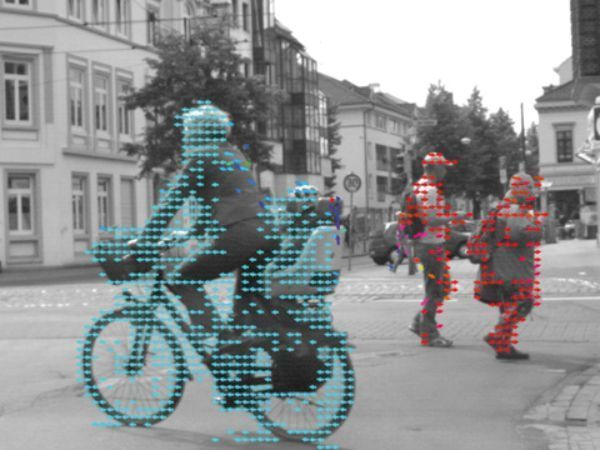
\includegraphics[width=0.8\linewidth]{Figures/opticalflow.jpeg}
 \caption{Motion Vector in Video Codec.}
 \label{fig:opticalflow}
\end{figure*}
\begin{figure*}
\centering
 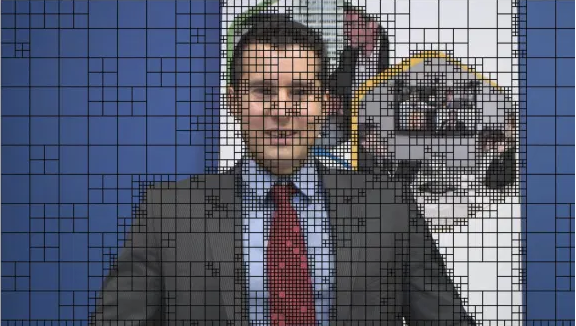
\includegraphics[width=0.8\linewidth]{Figures/macroblock.png}
 \caption{Macroblock in Video Encoder.}
 \label{fig:macroblock}
\end{figure*}
Figure \ref{fig:opticalflow} shows the optical flow (or motion vector) field of an image. Concentrate on the objects in the image above and the motion vectors drawn on them. Analyzing the motion vectors, we can see that a bicycle is moving towards the left while two pedestrians are moving towards the right. The speed of their motion is categorized by the magnitude of the motion vectors and their direction by the angel of the motion vectors. And it would be necessary to send the optical flow vector for every pixel to the video decoder.\\
 In video coding standard, a practical and widely-used method of motion compensate for movement of rectangular sections or 'block' of the current frame. The current frame is sub-devided in MxN blocks called macroblocks as shown in Figure \ref{fig:macroblock}. The following procedure is carried out for each block MxN samples in the current frame:
\begin{itemize}
\item Search an area in the reference frame (past or future frame) to find a 'matching' MxN-sample region. This process of finding the best match is known as motion estimation.
\item The chosen candidatge region becomes the predictor for the current MxN block and is subtracted from the current block to form a residual MxN block (motion compensation).
\item The residual block is encoded and transmited and the offset between the current block and the position of the candidate region (motion vector) is also transmitted. 
\end{itemize}
\begin{figure*}
\centering
 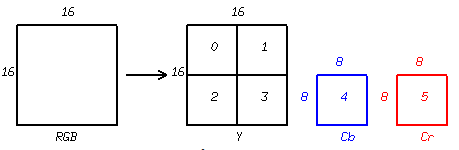
\includegraphics[width=0.8\linewidth]{Figures/yuv420.png}
 \caption{Macroblock (4:2:0).}
 \label{fig:yuv420}
\end{figure*}
	In H264/AVC standard, the macroblock, coressponding to a 16x16 pixel region of a frame is the basic unit for motion compensated prediction. In the RGB colour space, a colour image sample is represented by three numbers indicating the relative proportions of Red, Green and Blue. Computer display works naturally well in the RGB colour space. However, human eyes are more sensitive to luminance ( brightness ) than to colour. One can down sample an image by transforming the RGB to YCbCr representation and throw away some color components without causing much visual distortion. For example, in the 4:2:0 sampling format, Cb and Cr each has half the horizontal and vertical resolution of Y. Figure \ref{fig:yuv420} shows a 16x16 pixel macroblock represented in YCbCr 4:2:0 format. A macroblock of 16x16 pixels can be divided into 8x8 sample blocks. In the RGB representation, a macroblock has a total of 3x4 = 12 8x8 sample blocks ( four for each of the colors Red, Green and Blue ). In the YCbCr 4:2:0 format there are only six sample blocks, four for the Y component and 1 for each of Cb and Cr component.\\
  In  motion compensation, MV of a current block are correlated with the MVs of neighboring blocks in the current frame or in the earlier coded frames \cite{laroche2008rd}, \cite{jiang2019spatial}. While intra-picture prediction exploits correlations between spatially neighboring samples, inter-picture prediction makes use of temporal correlation between frames to derive a motion-compensated prediction (MCP) for a block of frame samples \cite{bross2014inter}.
\begin{figure*}
\centering
 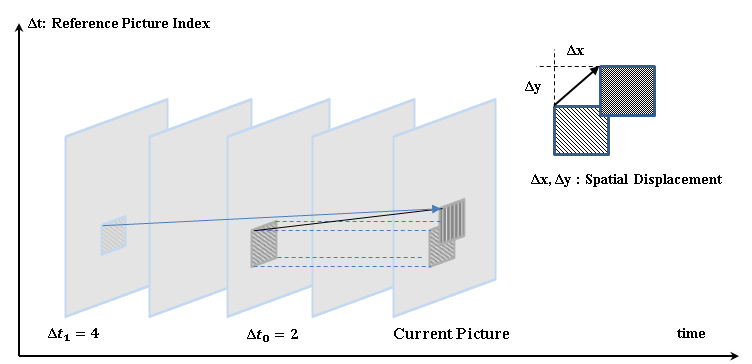
\includegraphics[width=0.8\linewidth]{Figures/mv.png}
 \caption{ Reference motion vectors in video coding.}
 \label{fig:mv}
\end{figure*}
For intra-prediction, we assume that neighboring blocks possibly correspond to the same moving object with similar motion and the motion of the object is not likely to abruptly change over time. Consequently, using MV in neighboring blocks as predictor reduces the size of the signaled motion vector difference. For this block-based MCP, a video image is divided into rectangular blocks. Figure \ref{fig:mv} shows the general concept of MCP based on a translational motion model. Using a translational motion model, the position of the block in a previously decoded picture is indicated by a motion vector $(\Delta x, \Delta y)$, where $\Delta x$ specifies the horizontal and $\Delta y$ the vertical displacement relative to the position of the current block. Note that the motion vectors $\Delta x$, $\Delta y$ could be of fractional sample accuracy to more accurately capture the movement of the underlying object. These MVs are coded by entropy coding and placed into a compressed bitstream for delivery to the video decoder, which uses MVs, along with one or more previously decoded pictures, to reconstruct the current image. On the other hand, H.264/AVC(Advanced Video Coding) in view of higher resolution, low bandwidth utilization and storage requirement becomes the popular video compression standard for surveillance video. In H.264/AVC, each video sequence is devided into groups of pictures (GOP), comprising at least one intra code I frame, uni-directionally predicted P frames and bi-directionally predicted B frames. Typically, the first frame in a GOP is intra coded I frame and follows by P, B frames. I frame uses raw data from camera, while other frames in a GOP ultilize the predictive coding involved motion vectors displacement. \\
%This is done by finding a displacement vector, i.e motion vector, for each block so that it optimises the rate-distortion requirements. As a result of the search criteria for 
\section{Compressed-Domain Based Moving Object Detection}
% Uncomment this line, when you have siunitx package loaded.
%The SI Units for dynamic viscosity is \si{\newton\second\per\metre\squared}.
%I'm going to randomly include a picture Figure~\ref{fig:minion}.


%If you have trouble viewing this document contact Krishna at: \href{mailto:kks32@cam.ac.uk}{kks32@cam.ac.uk} or raise an issue at \url{https://github.com/kks32/phd-thesis-template/}


%\begin{figure}[htbp!] 
%\centering    
%
\includegraphics[width=1.0\textwidth]{minion}
%\caption[Minion]{This is just a long figure caption for the minion in Despicable Me from Pixar}
%\label{fig:minion}
%\end{figure}
 As mentioned in last section, MVs are obtained for each motion block between the current and referenece frames. By minimising the prediction residual, the MVs represent the temporal displacement between the two block in the process of motion compression. Therefore, MV information indeed follow the real motion of objects and can be used for tracking.Therefore, MV information indeed follow the real motion of objects and can be used for tracking.\\
In recent studies, compressed-domain based video analytics methods  \cite{bombardelli2018efficient},\cite{khatoonabadi2012video} that rely on video coding artifact of compressed bitstreams, such as MVs, macroblock partition, and quantization coefficients, have been proposed. In \cite{bombardelli2018efficient}, the authors applied a probabilistic technique of computer vision for image separation, known as Graph Cut \cite{boykov2001fast}, modeling with MVs rather than pixels and adapted to the additional temporal dimension of video signals. Using MVs and a spatio-temporal Markov random field (ST-MRF) model that naturally integrates the spatial and temporal aspects of the object’s motion for tracking. In general, these approaches do not rely on pixels and studies by only using the codec’s MVs and block coding modes extracted bitstream through inexpensive partial decoding. In this manner, computing and storage requirements have been significantly reduced compared to “pixel-domain”.\\

\begin{figure*}
\centering
\subfloat[]
{
    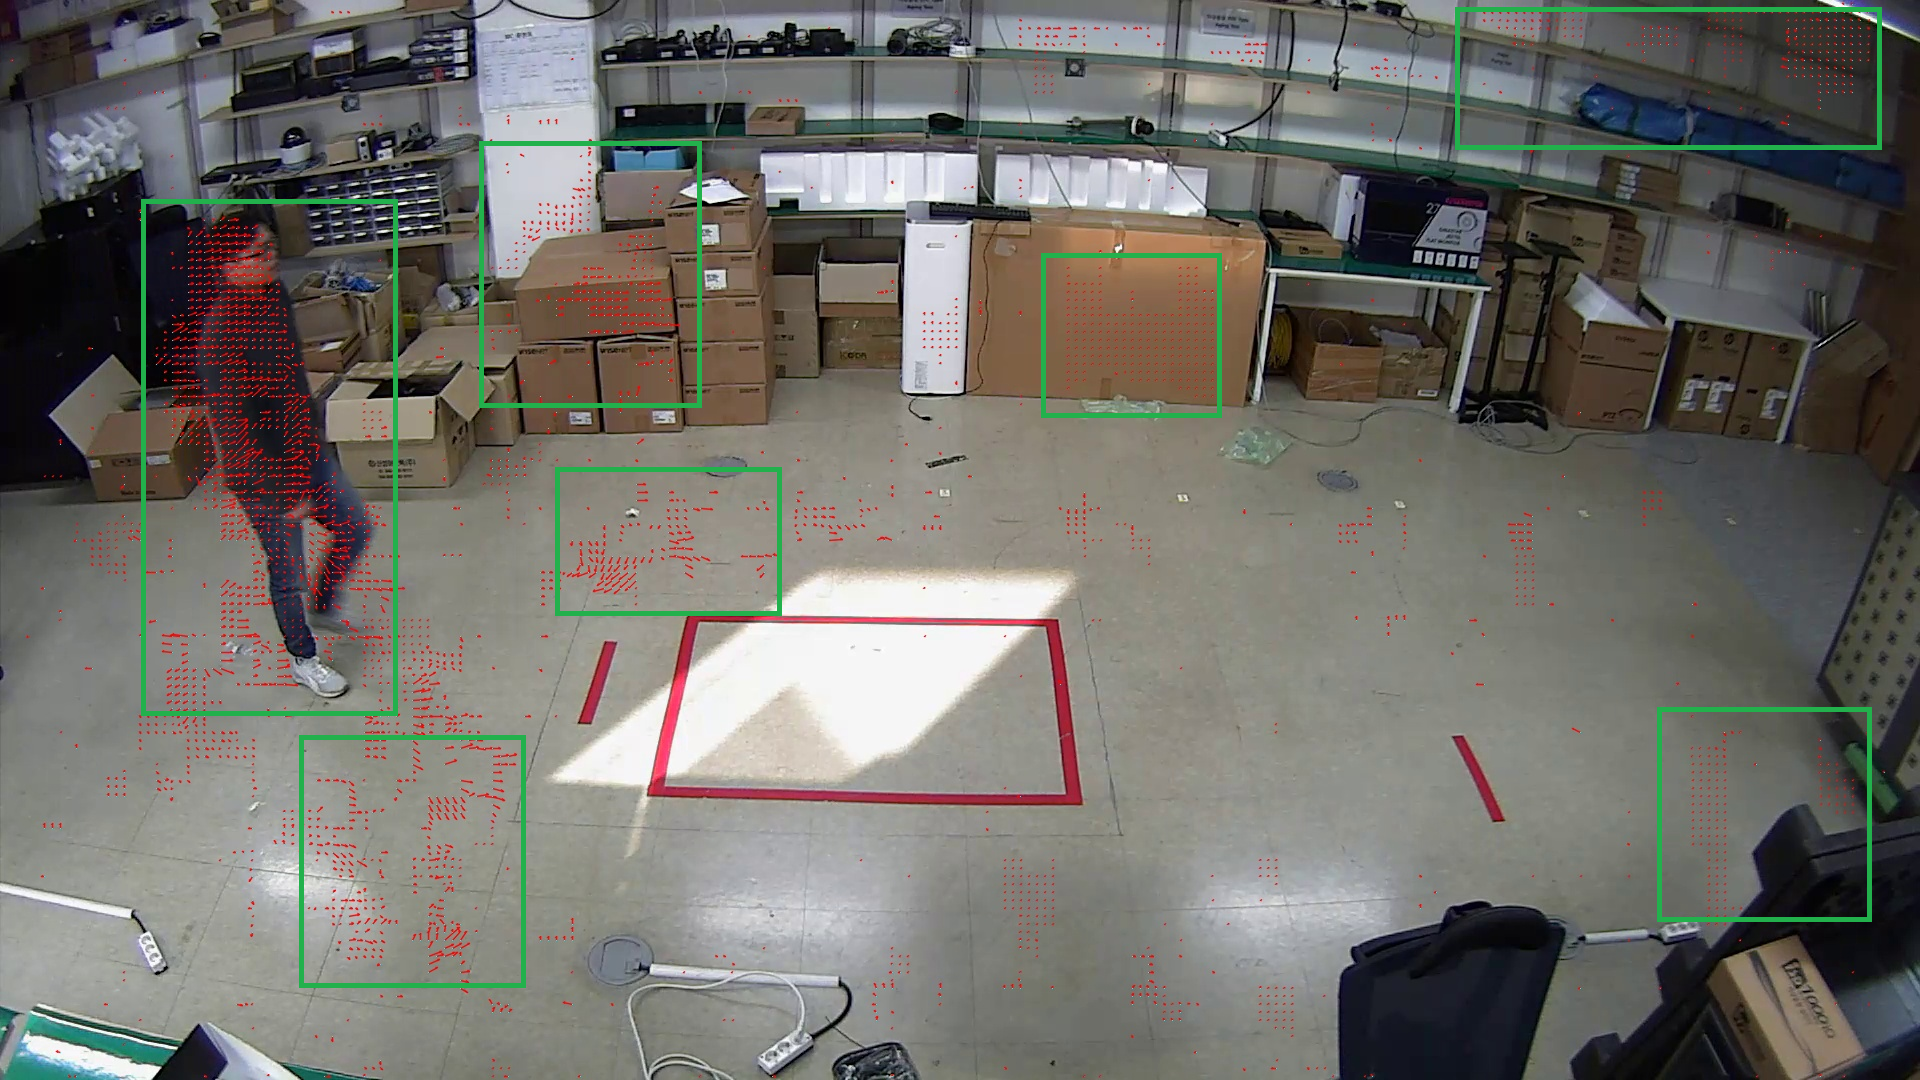
\includegraphics[width=0.5\linewidth]{Figures/noise.png}
}
\subfloat[]
{
    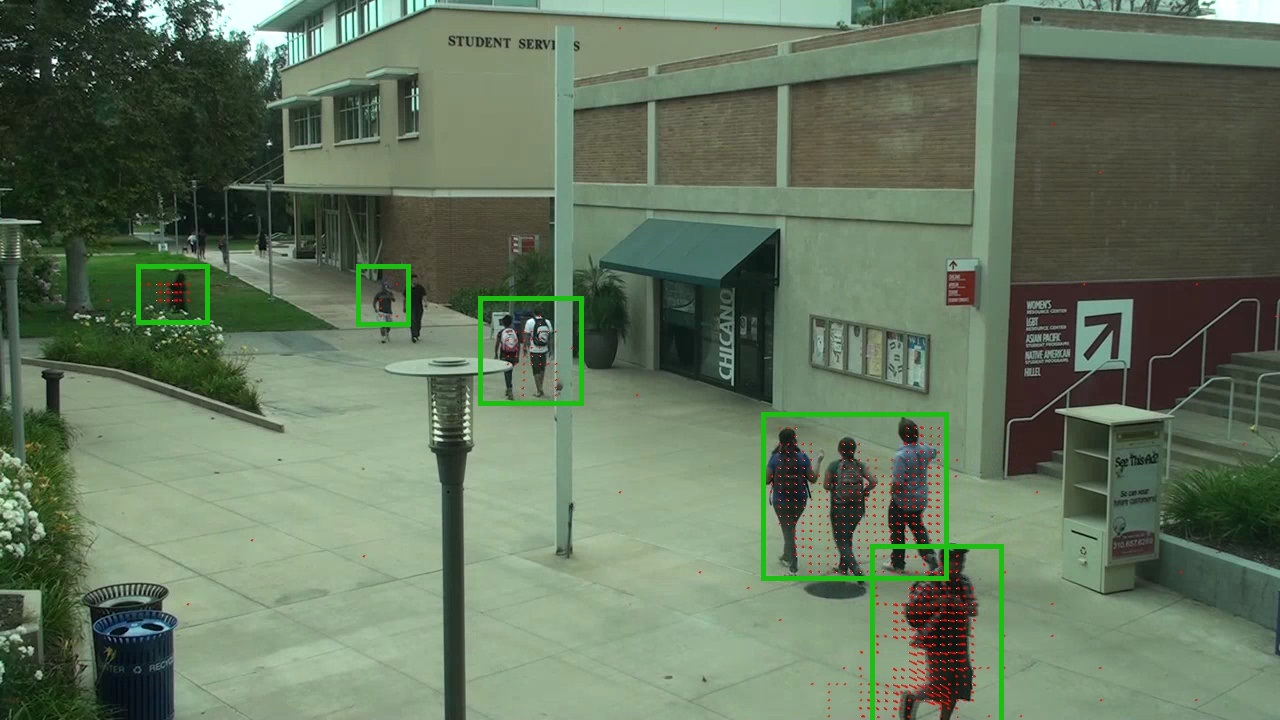
\includegraphics[width=0.5\linewidth]{Figures/34.jpg}
}
 \caption{ Example of motion vectors extraction.(a) Test video sequence from our recorded video, (b) Test video sequence from VIRAT.}
 \label{fig:noise}
\end{figure*}

The primary limitation of this approach is that it may lead to a noisy MV field that does not necessarily correspond with actual object movement of the object in the scene, as shown in Figure \ref{fig:noise}. The noisy MVs fail to provide useful information such as those attributed to illumination changes and background movement. The amount of noise MVs is relatively reduced compared to the correctly estimated MVs because noisy vectors are continuous and similar MVs from real moving objects. Another challenge of this approach is the lack of information about the object’s appearance such as color, edges and texture, because these features would require complete decoding of the compressed bitstream. In this study, our aim is to work in the “compressed domain” and uses only the MVs from the compressed bitstream to detect and track moving objects in video frames. 
%To apply the IoU-based object tracking algorithm \cite{rezatofighi2019generalized}, MVs are clustered into blobs and simply represented with object bounding boxes.

\section{Pixels-Domain Based Moving Object Detection}
Due to more reliable features that can be extracted from the pixel data, the majority of moving object detections require full decoding of the video stream. In pixels domain, a video analytics server analyzes the red-green-blue image to determine the appearance objects and spatial events. Ubiquitous real-time video analytics remains an open and exciting research problem, and it is fueled by the recent advantages of hardware and deep learning \cite{zeng2018background},\cite{chen2017pixel},\cite{babaee2018deep},\cite{wang2017interactive},\cite{patil2018msfgnet},\cite{ou2019moving}. There are two primary methods that are considered for moving object detection in pixels domain.
\subsection{Hybrid model of background subtraction and object classification based moving object detection}
\begin{figure*}
\centering
\subfloat[]
{
    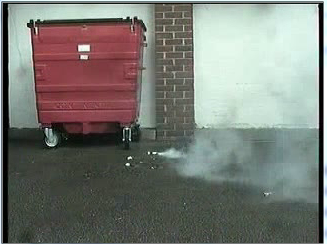
\includegraphics[scale=0.5]{Figures/input_img.png}
}
\subfloat[]
{
    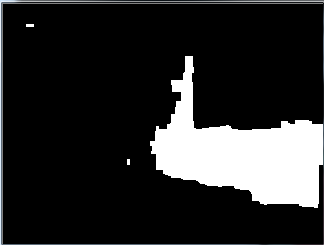
\includegraphics[scale=0.5]{Figures/fg_subtration.png}
}\\
\subfloat[]
{
    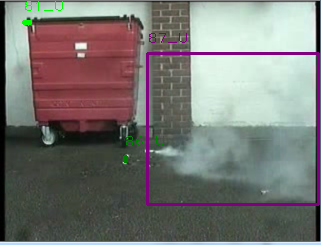
\includegraphics[scale=0.5]{Figures/blob_detection.png}
}
\subfloat[]
{
    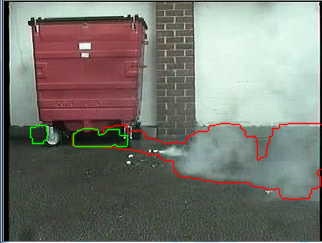
\includegraphics[scale=0.5]{Figures/smoke_region.png}
}
\caption{Smoke detection process: (a) input image, (b) foreground subtraction, (c) blob detection, (d) smoke classification }
\label{fig:bgmethod}
\end{figure*}
\begin{figure*}
\centering
 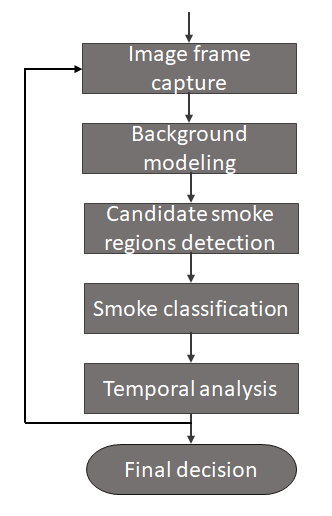
\includegraphics[width=0.3\linewidth]{Figures/smoke.jpg}
 \caption{Flow chart of our video- based smoke detection algorithm.}
 \label{fig:smoke}
\end{figure*}
The background subtraction method \cite{lee2012adaptive}\cite{stauffer1999adaptive} subtracts the current frame and background image to eliminate an image’s background, and then detects moving targets based on gray value differences. This method is the most commonly used object detection technique. There are a number of methods that have been for building the background model, e.g.,  \cite{lu2008improved} proposed a novel real-time motion detection algorithm that integrates the temporal differencing method, double background filtering method, optical flow method, and morphological processing methods to obtain excellent performance. Moreover, the authors of \cite{stauffer1999adaptive} discussed modeling each pixel as a grouping of Gaussians using an on-line approximation to renew the model. The Gaussian distributions of the adaptive mixture model were then assessed to determine which model can be presumed to be obtained from a background process. This method’s advantage is its simple implementation, low computational resource requirements, robustness in the presence of environmental noise, and dynamic background. However, it has limitations with shadows, background changes, as well as object localization and classification. Furthermore, object detection based on the background model cannot detect the individual objects in a group or a block object. In general, the aim of background subtraction is to separate foreground images from background ones in the form of blobs, followed by an object classification process. The detected blobs then help classify each blob into subclasses, as shown in Figure \ref{fig:bgmethod}, which shows the complete process of this approach is to perform smoke detection with the detail of flow-char is drawn in Figure \ref{fig:smoke}. Fortunately, deep learning, a relatively new technique in machine learning, enables very accurate classification of images using convolutional neural networks (CNNs) \cite{lecun2010convolutional}\cite{jarrett2009best}\cite{lee2009convolutional}. The capacity of CNNs can be controlled by varying their depth and breadth; moreover, they make strong and mostly correct assumptions about the nature of images (i.e., stationarity of statistics and locality of pixel dependencies). For example, by combining CNN and transfer learning, the authors of \cite{hussain2018study} achieved an average accuracy of 70.1\% using the CIFAR-10  \cite{krizhevsky2009learning} dataset.

\subsection{Deep Learning based Moving Object Detection}
\label{subsec:frameworks}
\begin{figure*}
\centering
\subfloat[]
{
    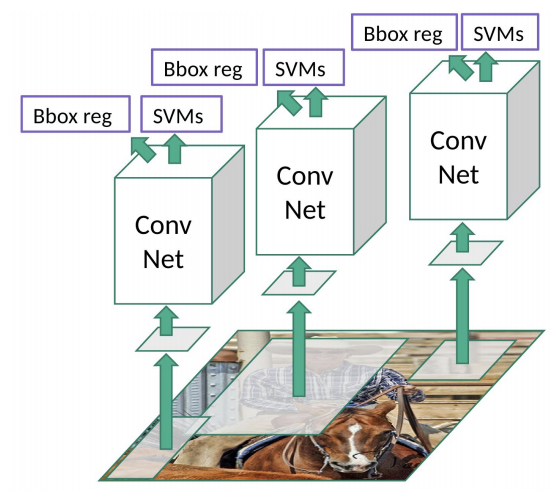
\includegraphics[scale=0.3]{Figures/rcnn.png}
}
\subfloat[]
{
    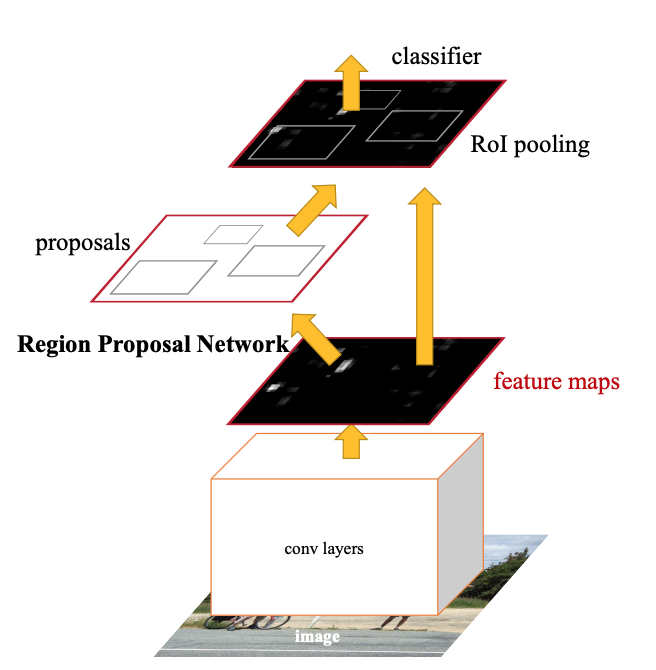
\includegraphics[scale=0.45]{Figures/faster_rcnn.png}
}\\
\subfloat[]
{
    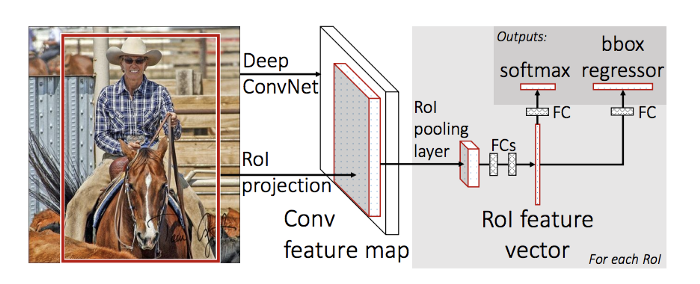
\includegraphics[scale=0.5]{Figures/fast_rcnn.png}
}
\caption{CNN based Object Detection Framework Structure.(a) RCNN, (b) Faster-RCNN, (c)Fast-RCNN.}
 \label{fig:cnn}
\end{figure*}

\begin{figure*}
\centering
 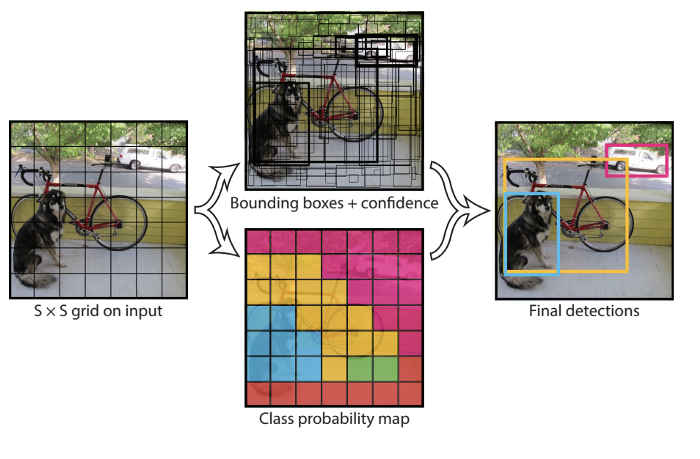
\includegraphics[width=0.8\linewidth]{Figures/yolo.png}
 \caption{YOLO Structer.}
 \label{fig:yolo}
\end{figure*}

Hybrid background subtraction and deep learning classification enhance the system’s accuracy; however, there are issues with detection of individual objects in a group or blocked objects and the background changes by the lighting condition and the environmental noise. Hence, the usage of deep learning is considered for robust object detection tasks. We have identified three primary object detection methods using deep learning:
\begin{itemize}
\item R-CNN, Fast R-CNN, Faster R-CNN
\item You Only Look Once (YOLO)
\item Single Shot Detectors (SSDs) 
\end{itemize}
R-CNN \cite{girshick2014rich} uses selective search \cite{uijlings2013selective} to extract several regions, called region proposals, from the image; it then attempts to classify a large number of regions. Each region proposal is placed into CNNs to extract features, which are fed to a support vector machine to classify the presence of object within the candidate region proposal as shown in Figure \ref{fig:cnn}(a). The limitation of this method is that it requires a large amount of time to train and deploy networks because it has to classify multiple region proposals per image. Fast R-CNN \cite{girshick2015fast} solves the limitations of R-CNN by putting the entire image into the CNNs to generate a convolutional feature map and identify the region of proposals based on the map, thus reducing the number of classified region of proposals as drawn in Figure \ref{fig:cnn}(c). Both R-CNN and Fast R-CNN use selective search to identify the region proposals. Selective search is a slow and tedious process that affects the network’s performance. Faster R-CNN \cite{ren2015faster} was proposed to allow the network to learn the region proposals as shown in Figure \ref{fig:cnn}(b); it uses a separate network to predict the region proposals rather than use a selection search algorithm on the feature maps output using the CNN layer. YOLO \cite{redmon2016you} is an object detection system targeted for real-time processing. Unlike R-CNN, Fast R-CNN and Faster R-CNN, which use regions to localize the object within the image, YOLO use a single neural network to predict the bounding boxes and the class probabilities for these boxes during training and test periods. Hence, YOLO only examines the input picture once to predict the presence and location of objects. YOLO divides the input image into an SxS grid, and multiple bounding boxes can exist within each grid. For each bounding box, the network outputs a class probability and offset value for the bounding box. The bounding boxes with class probabilities above a certain threshold value are then selected and used to locate the object within the image as shown in Figure \ref{fig:yolo}. Specially, YOLOv3 network architecture has 24 convolutional layers, followed by two fully connected layers as shown in Figure \ref{fig:yolov3}. The initial convolutional layers of the network extract feature from the image, while the fully connected layers predict the output probabilities and coordinates. According to performance comparison in \cite{redmon2018yolov3}, YOLOv3 is faster (45 frames per second (FPS)) than the other object detection algorithms. Faster R-CNN is more accurate than YOLOv3 (a mean average precision (mAP) of 73.2, as compared to 63.4); however, YOLOv3 is considerably faster than Faster R-CNN (FPS of 45, as compared to 7). Therefore, SSDs  \cite{liu2016ssd} were released as a balance between these two methods. Compared to YOLO, an SSD runs an input image through a convolutional network only once and computes a feature map. Then, a small 3 × 3 sized convolutional kernels are run on this feature map to predict the bounding boxes and categorization probability. Moreover, SSD uses anchor boxes at various aspect ratios comparable to Faster-RCNN and learns the off-set to a certain extent compared to learning the box. The SSD is able to detect objects of multiple scales because every convolutional layer function at a diverse scale. Compared to the YOLOv3 method \cite{redmon2018yolov3}, the SSDs attain similar accuracy but run slower. In this study, YOLOv3 was applied to robust human detection at cloud servers for our implementation. 

\begin{figure*}
\centering
 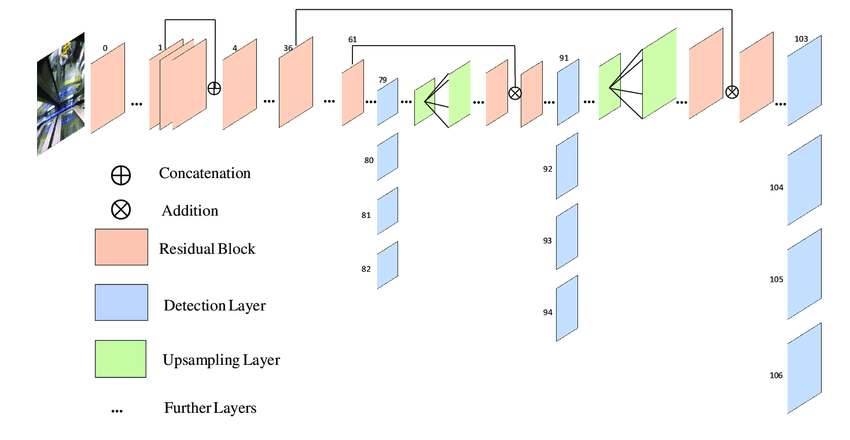
\includegraphics[width=1.0\linewidth]{Figures/yolov3.png}
 \caption{YOLOv3 Network Model.}
 \label{fig:yolov3}
\end{figure*}
